% documentation_EN.tex — WAC (Windows Artefacts Collector) user manual, English edition.
% The French edition is documentation_FR.tex, in this folder: both are maintained
% together, section for section.
%
% Build (XeLaTeX, two passes for the cover page and the table of contents):
%     latexmk -xelatex documentation_EN.tex
% The cover page is ../cover_EN.png, generated from the French one by
% ../translate-cover.py.

\documentclass[11pt,a4paper,oneside]{report}

% ---------------------------------------------------------------- fonts, language
\usepackage{fontspec}
\usepackage[british]{babel}
\setmainfont{Noto Sans}
\setmonofont{DejaVu Sans Mono}[Scale=0.84]

% ---------------------------------------------------------------- layout
\usepackage[top=26mm,bottom=26mm,left=24mm,right=22mm,headheight=14pt]{geometry}
\usepackage{graphicx}
\graphicspath{{../}}
\usepackage{xcolor}
\usepackage{tikz}
\usepackage{booktabs,tabularx,longtable,array}
\usepackage{enumitem}
\usepackage{fancyhdr}
\usepackage{titlesec}
\usepackage[most]{tcolorbox}
\usepackage{listings}
\usepackage{url}
\usepackage{lastpage}
\usepackage[hidelinks,unicode,pdfpagelabels]{hyperref}

% Colours sampled from the cover page
\definecolor{marine}{HTML}{0A1A33}
\definecolor{bleu}{HTML}{2F6DB5}
\definecolor{accent}{HTML}{1F66D1}
\definecolor{fond}{HTML}{EEF3FA}
\definecolor{alerte}{HTML}{B3261E}
\definecolor{fondalerte}{HTML}{FBEDEC}
\definecolor{gris}{HTML}{5B6573}

\setlength{\parindent}{0pt}
\setlength{\parskip}{0.55em}
\linespread{1.08}
\setlist{itemsep=0.25em,topsep=0.35em}
\urlstyle{tt}
\renewcommand{\arraystretch}{1.25}
% Left-aligned table columns: justified narrow columns opened wide gaps
% between words.
\newcolumntype{L}[1]{>{\raggedright\arraybackslash}p{#1}}
% Monospaced file and field names cannot be hyphenated: let the line's spaces
% stretch instead.
\setlength{\emergencystretch}{3em}

% Headings
\titleformat{\chapter}[display]
  {\color{marine}\bfseries\raggedright}
  {\color{bleu}\large\MakeUppercase{\chaptertitlename}~\thechapter}
  {0.3em}
  {\Huge}[{\color{accent}\titlerule[2pt]}]
\titlespacing*{\chapter}{0pt}{0pt}{1.6em}
\titleformat{\section}{\color{marine}\Large\bfseries}{\color{bleu}\thesection}{0.8em}{}
\titleformat{\subsection}{\color{marine}\large\bfseries}{\color{bleu}\thesubsection}{0.7em}{}
\titleformat{\subsubsection}{\color{bleu}\normalsize\bfseries}{}{0em}{}

% Headers and footers
\pagestyle{fancy}
\fancyhf{}
\fancyhead[L]{\small\color{gris}WAC — User manual}
\fancyhead[R]{\small\color{gris}\leftmark}
% Footer: "Page N of M", readable. A bare, small, light-grey number went
% unnoticed.
\newcommand{\piedpage}{\small\color{marine}\textbf{Page \thepage}\ of \pageref*{LastPage}}
\fancyfoot[C]{\piedpage}
\renewcommand{\footrulewidth}{0.4pt}
\renewcommand{\footrule}{\hbox to\headwidth{\color{fond}\leaders\hrule height \footrulewidth\hfill}}
\renewcommand{\headrulewidth}{0.4pt}
\renewcommand{\headrule}{\hbox to\headwidth{\color{fond}\leaders\hrule height \headrulewidth\hfill}}
\renewcommand{\chaptermark}[1]{\markboth{#1}{}}
\fancypagestyle{plain}{\fancyhf{}\fancyfoot[C]{\piedpage}\renewcommand{\headrulewidth}{0pt}}

% Boxes
\newtcolorbox{note}[1][Keep in mind]{enhanced,breakable,colback=fond,colframe=bleu,
  boxrule=0pt,leftrule=3pt,arc=0pt,left=8pt,right=8pt,top=6pt,bottom=6pt,
  title={\bfseries #1},coltitle=bleu,colbacktitle=fond,attach title to upper={\par\smallskip}}
\newtcolorbox{attention}[1][Warning]{enhanced,breakable,colback=fondalerte,colframe=alerte,
  boxrule=0pt,leftrule=3pt,arc=0pt,left=8pt,right=8pt,top=6pt,bottom=6pt,
  title={\bfseries #1},coltitle=alerte,colbacktitle=fondalerte,attach title to upper={\par\smallskip}}

% Code
\lstset{basicstyle=\ttfamily\small,columns=fullflexible,keepspaces=true,
  backgroundcolor=\color{fond},frame=l,framerule=3pt,rulecolor=\color{bleu},
  xleftmargin=9pt,framexleftmargin=6pt,aboveskip=0.8em,belowskip=0.8em,
  breaklines=true,breakatwhitespace=false,showstringspaces=false,
  literate={é}{{\'e}}1 {è}{{\`e}}1 {à}{{\`a}}1 {ê}{{\^e}}1 {ô}{{\^o}}1 {ç}{{\c c}}1
           {É}{{\'E}}1 {—}{{---}}1 {’}{{'}}1 {…}{{...}}1 {«}{{\guillemotleft}}1 {»}{{\guillemotright}}1}

% Shortcuts
\newcommand{\wac}{\textsc{wac}}
\newcommand{\opt}[1]{\texttt{-{}-#1}}
\newcommand{\champ}[1]{\texttt{#1}}
\newcommand{\fichier}[1]{\texttt{#1}}

\hypersetup{pdftitle={WAC — User manual},
  pdfauthor={Aerospace Cyber Defence Centre of Excellence (CEC)},
  pdfsubject={Windows artefact collection software for digital forensic investigation}}

\begin{document}

% ============================================================ COVER PAGE
\pagenumbering{roman}
\begin{titlepage}
\thispagestyle{empty}
\begin{tikzpicture}[remember picture,overlay]
  \node[inner sep=0pt] at (current page.center)
    {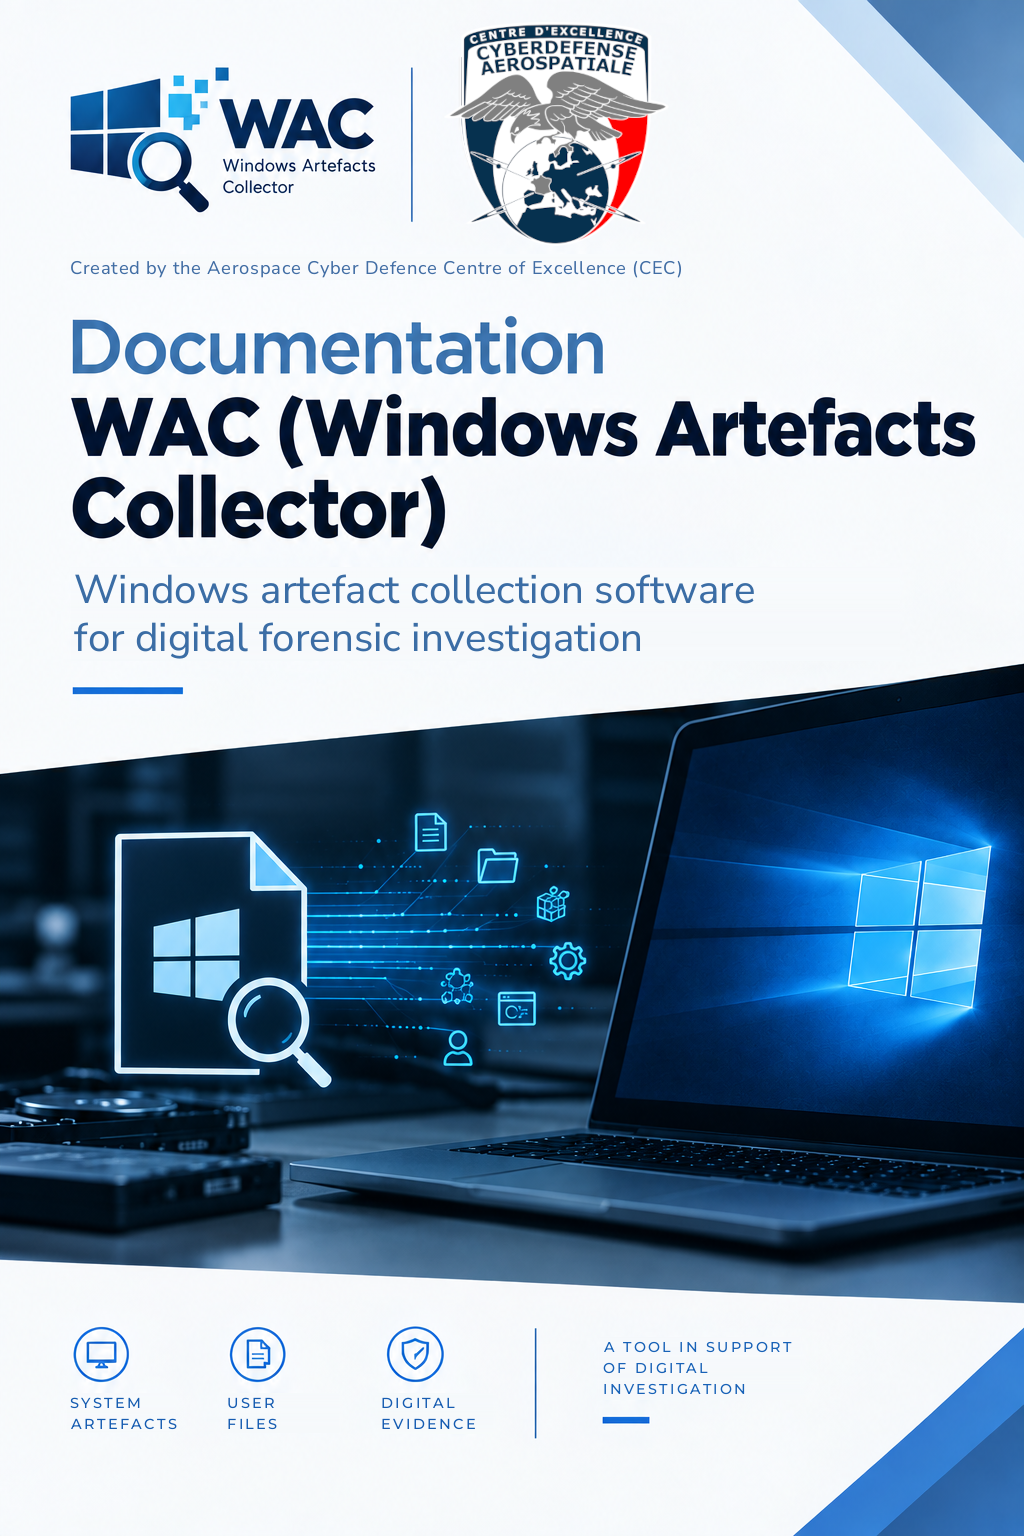
\includegraphics[width=\paperwidth]{cover_EN.png}};
\end{tikzpicture}
\end{titlepage}

% ============================================================ INFORMATION PAGE
\thispagestyle{empty}
\vspace*{\fill}
{\color{marine}\Large\bfseries WAC — Windows Artefacts Collector}\par
{\color{bleu}User manual}\par
\medskip
\begin{tabular}{@{}ll@{}}
Software version & 1.3.1 \\
Document edition & September 2026 \\
Publisher & Aerospace Cyber Defence Centre of Excellence (CEC) \\
          & French Air and Space Force Academy, Air Base 701, Salon-de-Provence \\
\end{tabular}

\bigskip
{\small\color{gris}This document describes how to use \wac{}: preparing and
running a collection, reading and verifying its results, and the traces it
leaves on the examined machine. The figures quoted were measured on a
Windows~11 test virtual machine; they are orders of magnitude, not
commitments.}
\vspace*{2cm}
\clearpage

% Numbering starts at 1 with the table of contents; only the cover page and the
% information page, which have no footer, are left out of it.
\pagenumbering{arabic}
\tableofcontents

% ============================================================ 1
\chapter{Overview}

\section{What WAC is for}

\wac{} collects, from a running Windows computer, the artefacts a digital
investigation needs: registry, event logs, Prefetch files, shortcuts and jump
lists, scheduled tasks, services, accounts, processes and sessions. It delivers
them as \textbf{JSON} files, ready to be analysed or fed into a processing
pipeline.

It runs from a USB stick, without installation, and writes everything it
produces to that stick.

\section{The guiding principle: a minimal footprint}

Examining a machine changes it. Every tool leaves traces: opened files whose
last-access date changes, services that write to the logs when solicited,
registry keys read through the API. These traces mix with the ones being looked
for.

\wac{} is designed so that what it leaves behind is as close to nothing as the
task allows, and so that \textbf{whatever it cannot avoid is written down}.
In practice:

\begin{itemize}
  \item the disk is read \textbf{directly}, read-only, without the system
        opening any file: no access date is modified;
  \item no key of the machine's registry is opened: the hives are copied, then
        read on the copy;
  \item no Volume Shadow Copy, no COM or WMI call, no logging service is
        solicited;
  \item nothing is written to the examined disk;
  \item every operation is recorded, with the trace it is expected to leave, in
        \fichier{investigation.json}.
\end{itemize}

\section{What WAC does not do}

\begin{itemize}
  \item \wac{} \textbf{does not analyse}: it collects and formats. Interpretation
        is the analyst's.
  \item It does not make a full disk image: it extracts the files that hold
        artefacts.
  \item It does not capture memory. The only volatile data collected are the
        process list, the open sessions and the state of the services.
\end{itemize}

% ============================================================ 2
\chapter{How it works}

\section{Reading the disk directly}

\wac{} opens the volume (\path|\\.\C:|) read-only, walks the NTFS file table
(\path|$MFT|) itself and extracts the content of the files it needs. The system
sees no file being opened: no access date updated, no directory walked, no
lock.

This reading handles the NTFS features Windows normally hides:

\begin{description}[style=nextline,leftmargin=1.2em]
  \item[NTFS compression] Windows~11 compresses, among others, the event log
        folder. \wac{} decompresses it itself.
  \item[Compact OS (WOF)] The system binaries of Windows~10 and~11 are stored
        compressed in a hidden stream; seen through the API, they look ordinary.
        \wac{} decompresses them (XPRESS variants).
  \item[Split attributes] A heavily fragmented file has its information spread
        over several records; \wac{} gathers them.
  \item[Preallocated files] Beyond the valid data length, NTFS returns zeros,
        even if the disk still holds remnants of former files. \wac{} does the
        same: the extracted content is the one any ordinary acquisition would
        see, and so is its fingerprint.
\end{description}

\section{Exhibit store and working copy}

A digital exhibit is never examined on itself: a copy is taken and sealed, and
the work is done on a second copy. If the analysis damages something, the sealed
copy remains and the operation can be redone.

\wac{} applies this procedure to \textbf{every} extracted file, including those
it does not modify. The two directories keep their French names in the output:

\begin{description}[style=nextline,leftmargin=1.2em]
  \item[\fichier{exhibits/} — the exhibit store] the raw copies, as read from
        the volume. This directory is never reopened for writing after
        extraction. It holds the manifest identifying each exhibit, and the
        manifest's seal.
  \item[\fichier{working/} — the working copy] copied from the exhibit store and
        verified by fingerprint. The only modifications (replay of the hives'
        transaction logs) are made here, and every collector reads from here.
\end{description}

\begin{note}
Every extracted file is therefore written \textbf{twice} to the collection
medium. Plan for the space (see section~\ref{sec:place}).
\end{note}

\section{Registry hives and transaction logs}

A hive copied from a running machine lacks its latest changes: they are still in
its transaction logs (\fichier{.LOG1}, \fichier{.LOG2}). \wac{} extracts these
logs and \textbf{replays them onto the working copy}, so that the analysis bears
on the machine's actual state.

Everything \wac{} writes onto a copy can be undone: before the replay, the
original content of every replaced page is saved in an undo journal
(\fichier{<hive>.undo}). The raw copy stays intact in the exhibit store.

\section{Two-pass extraction}

Where each user's hives live is recorded in the \fichier{SOFTWARE} hive. \wac{}
therefore first extracts the machine's hives (\fichier{SYSTEM},
\fichier{SOFTWARE}, \fichier{SAM}, \fichier{Amcache}), reads the profile list in
the copy of \fichier{SOFTWARE}, then extracts each profile's hives
(\fichier{ntuser.dat}, \fichier{usrClass.dat}).

Nothing is assumed about \fichier{C:}: the system drive is detected, and a
profile on another disk (for instance \path|D:\Users\...|) is read on its own
volume.

\section{What is still read live}

Three pieces of information describe the very moment of the collection and are
held in no file. They are read live, with a single query each:

\begin{itemize}
  \item the running \textbf{processes} (a kernel snapshot);
  \item the open \textbf{sessions};
  \item the \textbf{current state of the services} (their configuration is read
        from the copied hive).
\end{itemize}

% ============================================================ 3
\chapter{Preparing a collection}

\section{Requirements}

\begin{itemize}
  \item Windows~10 or later, 64-bit. \wac{} checks it at start-up.
  \item \textbf{Administrator rights}: reading a volume directly requires them.
        \wac{} checks this too.
  \item \textbf{NTFS} volumes. A file on another file system (CD-ROM, FAT stick)
        cannot be read directly; it is reported as unread, never opened another
        way.
\end{itemize}

\section{The collection medium}\label{sec:place}

\wac{} runs from the collection medium (usually a USB stick) and writes all its
results there. Choose an \textbf{empty} medium, preferably USB~3: writing is the
most expensive part of a collection.

The space needed depends on the options. Orders of magnitude measured on an
ordinary Windows~11 installation, for the raw copies alone:

\begin{center}
\begin{tabular}{@{}L{9.6cm}r@{}}
\toprule
Content & Size of the raw copies \\
\midrule
Hives, Prefetch, shortcuts, jump lists (always) & about 200 to 350~MB \\
Event logs and their message binaries (\opt{events}) & about 250~MB \\
Referenced binaries not authenticated as Microsoft's (\opt{binary}) & a few hundred MB \\
\bottomrule
\end{tabular}
\end{center}

Since every copy is written twice (exhibit store and working copy),
\textbf{double these figures}. A full collection (\opt{events} \opt{binary})
thus takes about 1.5 to 2~GB on an ordinary installation.

\wac{} checks the location \textbf{before its very first write} and refuses to
start:
\begin{itemize}
  \item if the working directory already holds files — an earlier collection
        would be analysed instead of this one;
  \item if the free space is clearly insufficient.
\end{itemize}
If space runs out while binaries are being collected, they are hashed without
being copied, and the investigation log says so.

\section{Before going on site}

\begin{itemize}
  \item Use a \textbf{new output folder} for each machine (option
        \opt{output}).
  \item Note the time of the intervention and the operator's identity: \wac{}
        records them too, but an independent record is useful.
  \item Keep in mind that plugging the stick in and running \wac{} leave
        unavoidable traces (chapter~\ref{chap:traces}): they are known and
        documented, so that they are not mistaken for the activity under
        study.
\end{itemize}

% ============================================================ 4
\chapter{Running a collection}

\section{Command line}

Open a command prompt \textbf{as administrator}, move to the collection medium,
then run:

\begin{lstlisting}
WAC.exe [--events] [--binary] [--dump] [--output=folder] [--loglevel=N] [--debug]
\end{lstlisting}

Every option is optional and disabled by default.

\section{Options}

\begin{longtable}{@{}>{\ttfamily}L{3.2cm}L{11.2cm}@{}}
\toprule
\normalfont\bfseries Option & \bfseries Effect \\
\midrule
\endhead
-{}-events & Extracts and parses the event logs (\fichier{.evtx}), and rebuilds
  each event's readable message from its provider's resources. Adds about
  250~MB of copies. \\
-{}-binary & Fingerprints (MD5, SHA-1, SHA-256) every file referenced by an
  artefact, by reading the disk directly. Referenced executables, libraries,
  drivers and scripts are also \textbf{collected} into the exhibit store. See
  section~\ref{sec:binary}. \\
-{}-dump & Adds the raw hexadecimal value of shellbag and \fichier{.lnk} shortcut
  items, for later decoding. \\
-{}-output=folder & Output folder, relative to the current directory. Default:
  \fichier{output}. \\
-{}-loglevel=N & Enables a detailed text log in the current directory, named
  after the program run (\fichier{WAC.exe.log} for \fichier{WAC.exe}): 0~none,
  1~per artefact type, 2~per artefact, 3~per sub-function (debugging). \\
-{}-debug & Prints the NTFS reader's trace on standard error (path resolution,
  index blocks, cluster runs). For diagnosis only. \\
-{}-help, /? & Shows the help. \\
\bottomrule
\end{longtable}

\section{Examples}

Standard collection:
\begin{lstlisting}
E:\> WAC.exe --output=accounting-pc-01
\end{lstlisting}

Full collection, with logs, binaries and a detailed log:
\begin{lstlisting}
E:\> WAC.exe --events --binary --output=accounting-pc-01 --loglevel=2
\end{lstlisting}

\section{The \opt{binary} option}\label{sec:binary}

A fingerprint is enough to query a public database (VirusTotal, for instance)
\textbf{without sending it the file}. But it says nothing about a binary nobody
knows — precisely the one that matters to the investigation — and a binary left
behind may be gone by the time a detection comes in. This is why \opt{binary}
also copies potential payloads:

\begin{itemize}
  \item \textbf{collected}: \fichier{exe}, \fichier{dll}, \fichier{sys},
        \fichier{ocx}, \fichier{cpl}, \fichier{scr}, \fichier{drv},
        \fichier{efi}, \fichier{com}, \fichier{msi} and the scripts
        \fichier{ps1}, \fichier{psm1}, \fichier{bat}, \fichier{cmd},
        \fichier{vbs}, \fichier{vbe}, \fichier{js}, \fichier{jse},
        \fichier{wsf}, \fichier{wsh}, \fichier{hta};
  \item \textbf{collected as well}: Office documents \textbf{able to carry
        macros}, an intrusion vector as common as an executable — legacy binary
        formats (\fichier{doc}, \fichier{xls}, \fichier{ppt}, \fichier{pps},
        \fichier{dot}, \fichier{xlt}, \fichier{pot}), ``m'' formats
        (\fichier{docm}, \fichier{dotm}, \fichier{xlsm}, \fichier{xltm},
        \fichier{pptm}, \fichier{potm}, \fichier{ppsm}), \fichier{xlsb}, add-ins
        (\fichier{xla}, \fichier{xlam}, \fichier{xll}, \fichier{wll},
        \fichier{ppa}, \fichier{ppam}), Publisher (\fichier{pub}), Visio
        (\fichier{vsd}, \fichier{vsdm}, \fichier{vstm}, \fichier{vssm}) and
        Access (\fichier{mdb}, \fichier{accdb}, \fichier{accde}). They appear in
        the traces as targets of shortcuts or jump lists, or among the files
        loaded by Word or Excel in their Prefetch;
  \item \textbf{only hashed}: other documents and data files, including
        \fichier{docx}, \fichier{xlsx} and \fichier{pptx}, which cannot contain
        macros. Copying them would turn the collection into a copy of the
        user's files.
\end{itemize}

The referenced files come from processes, services (binary and DLL), scheduled
tasks, files loaded by programs (Prefetch), Shimcache, Amcache, and targets of
shortcuts and jump lists. Each file is read only once, however many artefacts
cite it, and \textbf{identical content is stored only once}: the other paths
appear in the manifest as exhibits sharing that content
(\champ{SharedExhibit}).

\subsection*{Authentic Microsoft binaries: hashed, not collected}

Most referenced binaries are Windows components, identical on every machine of
the same build. Their origin can be proven on the machine itself, with no list
to carry: Windows' \textbf{catalogs} (\path|System32\CatRoot|), signed by
Microsoft, list the fingerprint of every system file; individually signed
binaries (Edge, OneDrive, Office) carry an \textbf{embedded signature}. A
binary authenticated this way is hashed without being collected; every other one
is collected — including a system binary replaced by an attacker, whose
fingerprint no longer matches.

This check leaves \textbf{no trace}: catalogs and binaries are read directly
from the disk, and the cryptographic verification is done in memory by \wac{},
up to Microsoft root certificates embedded in the executable. No service is
solicited, the machine's certificate store is not consulted, and revocation is
not checked online.

Only signers Microsoft uses for its own code are accepted. \textbf{Third-party}
drivers certified by Microsoft (signers ``Hardware Compatibility Publisher'' and
``Early Launch Anti-malware Publisher'') are still collected: a vulnerable but
signed driver is a classic attack path.

The catalogs that justified not collecting a file go into the exhibit store, so
that a third party can redo the check. In the artefact files, the
\champ{Signature} field (or \champ{ServiceDllSignature},
\champ{SignatureTarget}\ldots) states the authentication used, for instance
``\texttt{Microsoft (catalogue Package\_xxx.cat)}'' or
``\texttt{Microsoft (signature intégrée)}'' (embedded signature).

\textbf{Scripts} are authenticated the same way: by Windows' catalogs and, for
PowerShell (\fichier{ps1}, \fichier{psm1}, \fichier{psd1},
\fichier{ps1xml}\ldots), by their embedded signature block
(\texttt{\# SIG \# Begin signature block}). A Windows Script Host script
(\fichier{vbs}, \fichier{js}, \fichier{wsf}) signed only within its text, and
not by a catalog, is still collected.

On the test machine, this check brings collection down from 2,131 binaries
(3.3~GB) to 92 (335~MB), without lengthening the collection; the scripts still
collected are the unsigned ones.

Since reading is direct, collecting leaves no more trace than hashing — it only
takes space on the medium.

\section{What the screen shows}

\wac{} displays each step, followed by \texttt{OK} or an error message. A failed
step does not stop the collection: whatever is accessible is gathered, and
whatever is missing is recorded.

\begin{lstlisting}
[PREREQUISITE VERIFICATION]
 - Check OS >= Windows 10 : OK
 - Check administrator rights : OK
 - Checking the collection medium : OK
[SEARCHING FOR ARTIFACTS IN WINDOWS API]
 - Extraction of SESSIONS: OK
 - Extraction of PROCESS: OK
[RAW EXTRACTION]
 - Extracting system hives (raw NTFS) : OK
 - loading the HKLM\SYSTEM key : OK
 - loading the HKLM\SOFTWARE key : OK
 - Listing USER PROFILES (SOFTWARE hive) : OK
 - Extracting user hives (raw NTFS) : OK
 - Extracting file artefacts (raw NTFS) : OK
[SEARCHING FOR ARTIFACTS IN THE REGISTRY]
 - Extracting USERASSIST Registry Keys : OK
   ...
[SEARCHING FOR ARTIFACTS IN FILES]
 - Extracting PREFETCHS : OK
   ...
[SEARCHING FOR ARTIFACTS IN EVENT LOGS]
 - Extraction of EVENTS: OK
[EXHIBIT STORE]
 - Copying collected binaries to the working directory : OK
 - Sealing the exhibit store (manifest + SHA-256) : OK
[INVESTIGATION LOG]
 - Writing investigation.json : OK
END, Time elapsed : 309 s
\end{lstlisting}

Sealing the exhibit store is the \textbf{last} operation on it: every exhibit,
including those added while the event logs are processed, is covered by the
manifest.

\section{Duration}

The duration depends mostly on the hardware (USB~2 or~3, disk, processor) and
the options. On the test virtual machine (NVMe disk): about 70~s with
\opt{events}, about 310~s with \opt{events} and \opt{binary}. On a USB stick,
writing dominates.

% ============================================================ 5
\chapter{The results}

\section{Layout}

\begin{lstlisting}
<output>/
  exhibits/            exhibit store: raw copies, never rewritten
    MANIFEST.json     identifies each exhibit and the collection
    MANIFEST.sha256   the manifest's fingerprint: its seal
    Windows/...        the exhibits, under their original paths
    Users/...
  working/             working copies (replayed hives)
  investigation.json   the collection log
  *.json               the artefacts
\end{lstlisting}

A file from a volume other than the system one is stored under
\path|_volume_D\...|; the JSON always gives the original path, with its real
drive letter.

\section{The exhibit store manifest}

\fichier{exhibits/MANIFEST.json} identifies the collection and each exhibit.

\subsection{Header}

\begin{description}[style=nextline,leftmargin=1.2em]
  \item[\champ{Tool}] tool name, command line, build date.
  \item[\champ{Host}] machine name, system drive, time zone of the suspect (read
        from its \fichier{SYSTEM} hive) and of the collecting machine.
  \item[\champ{Operator}] account that ran the collection, and whether it was
        elevated.
  \item[\champ{Custody}] procedure statement, start of extraction, time the
        manifest was written, number of exhibits and failures, total size, hash
        algorithms, volumes read (letter, serial number, file system).
\end{description}

\subsection{Each exhibit}

\begin{longtable}{@{}>{\ttfamily}L{4.2cm}L{10.2cm}@{}}
\toprule
\normalfont\bfseries Field & \bfseries Meaning \\
\midrule
\endhead
SourcePath & Original path, with drive letter. \\
ExhibitPath & Location of the raw copy, relative to the output folder. \\
Method & Collection method (direct NTFS reading, volume, purpose). \\
Result & \texttt{OK}, or the error code and message. Failures are listed in the
  manifest: a missing exhibit would read as one never looked for. \\
MD5, SHA1, SHA256 & The three fingerprints, computed while writing: they bear
  on what was read from the volume. \\
Bytes & Extracted size. \\
DeclaredBytes & Size declared by NTFS, present only when it differs from the
  extracted size (truncated extraction). \\
ValidDataBytes & Valid data length of a preallocated file (event logs): beyond
  it, the exhibit holds zeros by definition. \\
SharedExhibit & \texttt{true} when the content, identical byte for byte, is
  already stored under another exhibit: \champ{ExhibitPath} points to it. The
  source remains an exhibit in its own right, with its own path, \path|$MFT|
  entry and timestamps. \\
MftEntry & NTFS record number: identifies the file independently of its name. \\
Extracted(Utc) & When this exhibit was extracted. \\
SourceCreated, SourceModified, SourceMftModified, SourceAccessed & The four NTFS
  timestamps of the original file, in UTC and in the suspect's local time. \\
\bottomrule
\end{longtable}

\begin{note}[Why three fingerprints]
MD5 collisions have been producible at will since 2008, and SHA-1 ones since
2017: a single fingerprint no longer settles an identity dispute. Three
independent ones do.
\end{note}

\section{Verifying a collection}\label{sec:verif}

\subsection{The seal}

The manifest cannot hold its own fingerprint: it is in
\fichier{MANIFEST.sha256}. On Linux:

\begin{lstlisting}
$ cd output/exhibits
$ sha256sum -c MANIFEST.sha256
MANIFEST.json: OK
\end{lstlisting}

\subsection{Each exhibit}

The \fichier{verify-exhibits.ps1} script, supplied with this manual, checks the
seal, then the SHA-256 of every exhibit:

\begin{lstlisting}
PS> powershell -ExecutionPolicy Bypass -File verify-exhibits.ps1 -Output E:\output
Seal verified (CEB489A143AE29EB9E3BC836F3D565B744F036AE1F3A72A3447408F31F8A5B67)
1617 exhibit(s) verified, 0 mismatch(es)
\end{lstlisting}

Its exit code is~0 if everything matches, 1~otherwise.

\lstinputlisting[language={},caption={}]{verify-exhibits.ps1}

\section{The investigation log}

\fichier{investigation.json} traces the collection: tool and command line,
machine and time zones, operator, start, end and duration, then the
\textbf{ordered} list of operations. For each one:

\begin{description}[style=nextline,leftmargin=1.2em]
  \item[\champ{Seq}, \champ{TimestampUtc}, \champ{TimestampLocal}] rank and time;
  \item[\champ{Operation}, \champ{Target}] what was done, and on what;
  \item[\champ{Result}] the outcome;
  \item[\champ{Footprint}] the trace this operation is expected to leave on the
        examined machine.
\end{description}

This log makes it possible to compare, collection by collection, the expected
traces with those actually observed. It also flags a difference between the
suspect's time zone and the collecting machine's.

\section{The artefact files}

One file per artefact. The fields described are those emitted; a field without
a value is not emitted (see chapter~\ref{chap:lecture}).

\subsection{System and accounts}

\begin{description}[style=nextline,leftmargin=1.2em]
  \item[\fichier{OperatingSystem.json}] machine name and domain, Windows edition
        and version, installation date, current time, \textbf{boot time},
        uptime, time zone. \champ{BootTimeSource} says where the boot time comes
        from (kernel, or fallback estimate); \champ{ClockAdjustedSinceBootMs}
        gives the total clock corrections since boot — a few seconds is routine
        resynchronisation, a large value means a clock changed.
  \item[\fichier{users.json}] local accounts, read from the \fichier{SAM} hive:
        SID and RID, state, flags, logon and failure counts, dates of last
        logon, last failure, password change and account change, profile.
  \item[\fichier{Sessions.json}] sessions open at collection time: user, logon
        type, authentication package, start time.
  \item[\fichier{processes.json}] running processes: name, identifiers (and
        parent), owner, session, loaded modules and, with \opt{binary}, the
        executable's fingerprints.
  \item[\fichier{services.json}] services and drivers, configuration read from
        the hive: type, start mode, account, binary and hosted DLL, failure
        command, dependencies, last write of the key; current state; with
        \opt{binary}, fingerprints of the binary and of the DLL.
  \item[\fichier{ScheduledTasks.json}] scheduled tasks, read from their XML
        definitions: author, run-as account, state, last run and its result,
        triggers and actions (with \opt{binary}, fingerprints of the command).
\end{description}

\subsection{Program execution}

\begin{description}[style=nextline,leftmargin=1.2em]
  \item[\fichier{prefetchs.json}] Prefetch files: program, run count and times,
        volumes, and list of loaded files with their \path|$MFT| reference (and
        their fingerprints with \opt{binary}).
  \item[\fichier{amcache\_application\_files.json},
        \fichier{amcache\_applications.json}] Amcache inventory of executables
        and applications: path, publisher, version, dates.
  \item[\fichier{shimcache.json}] compatibility cache: path and modification date
        of the file. An entry proves the binary was present, not that it ran.
  \item[\fichier{bams.json}] last execution per program and per user
        (Background Activity Moderator).
  \item[\fichier{userassists.json}] programs launched from the user interface:
        count, focus time, last execution.
  \item[\fichier{muicache.json}] display names of executed programs.
  \item[\fichier{run.json}] programs started at boot or logon (Run keys), with
        the key's last write.
\end{description}

\subsection{Files and browsing}

\begin{description}[style=nextline,leftmargin=1.2em]
  \item[\fichier{recentdocs.json}] recent-document shortcuts: target, timestamps
        of the shortcut and of the target, volume (type, serial number, label),
        network path, shell item list.
  \item[\fichier{jumplistAutomaticDestinations.json},
        \fichier{jumplistCustomDestinations.json}] per-application jump lists,
        with the shortcuts they hold.
  \item[\fichier{shellbags.json}] folders browsed in Explorer, as a rebuilt
        tree.
  \item[\fichier{mrus.json}, \fichier{mruApps.json}] most-recently-used files
        and applications.
\end{description}

\subsection{Devices}

\begin{description}[style=nextline,leftmargin=1.2em]
  \item[\fichier{Usbstor.json}] USB storage devices known to the system.
  \item[\fichier{mounted\_device.json}] mapping between drive letters and
        devices.
\end{description}

\subsection{Event logs (\opt{events})}

\fichier{events.json} holds one object per event:

\begin{description}[style=nextline,leftmargin=1.2em]
  \item[\champ{EvtSystem*}] the system section: provider, identifier, level,
        task, keywords, creation time, record number, process and thread,
        channel, computer, user;
  \item[\champ{EvtEventData}] the event's data, as a list of \champ{Name} /
        \champ{Value} pairs;
  \item[\champ{EvtEventMessage}] the readable message, as Event Viewer would show
        it, rebuilt from the provider's resources collected on the machine;
  \item[\champ{EvtSourceLog}] the log file the event comes from. One channel can
        be carried by several files (current log and archives) whose record
        numbers overlap.
\end{description}

\begin{note}[Incomplete messages]
A \texttt{\%1}, \texttt{\%2}\ldots{} mark left in a message means the event does
not carry the expected data: it is kept visible so that the sentence does not
look complete. Not every provider ships message resources: their events then
have no \champ{EvtEventMessage}, but their data are complete.
\end{note}

% ============================================================ 6
\chapter{Reading the data}\label{chap:lecture}

\section{Timestamps}

Every date is emitted twice: \champ{X} in local time and \champ{XUtc} in UTC.
The local time is the \textbf{suspect's}, computed with the time zone read from
its \fichier{SYSTEM} hive — not the collecting machine's. Dates carry the
fraction of a second when the source provides it (down to a ten-millionth).

\section{A missing field is not an empty field}

A value with no source is not emitted at all. An empty key would read as a
failed read, and could not be told apart from ``the hive does not hold this
value''. What could not be read is recorded in \fichier{investigation.json}.

\section{Artefact not collected}

When a whole artefact could not be read, its file says so explicitly (the text
is produced in French):

\begin{lstlisting}
{
  "Artifact": "USBSTOR (registre)",
  "CollectionStatus": "NotCollected",
  "Error": "0x02 Le fichier spécifié est introuvable.",
  "Note": "La lecture de cet artefact a échoué : l'absence de données
           ci-dessus ne signifie PAS qu'aucune trace n'existe sur le système."
}
\end{lstlisting}

\begin{attention}
An empty artefact file and a ``NotCollected'' file do not say the same thing.
The first means no entry was found; the second, that the source could not be
read.
\end{attention}

\section{Undecoded data}

An item \wac{} cannot decode (unknown shell item, unrecognised extension block)
comes with its raw bytes in hexadecimal, so that an analyst can decode it later.
With \opt{dump}, the raw value of shellbags and shortcuts is always added.

\section{Paths}

Paths and values are delivered \textbf{as they are on the disk}, untransformed:
escaping happens only when the JSON is written.

% ============================================================ 7
\chapter{Traces left on the examined machine}\label{chap:traces}
\markboth{Traces on the examined machine}{}

Read this before using \wac{} on a case. This chapter lists what \wac{} does to
the machine, operation by operation, including what it cannot avoid.

\section{What WAC still does}

\begin{longtable}{@{}L{4.3cm}L{10.1cm}@{}}
\toprule
\bfseries Operation & \bfseries Trace \\
\midrule
\endhead
Direct volume reading & One access per volume actually read (usually one). No
  file opened, so no access date modified. If object-access auditing is enabled,
  opening the volume may be logged (Security 4656/4663). \\
Writing the results & On the collection medium only. Nothing is written to the
  examined disk. \\
Replaying hive logs & On the working copy only, with an undo journal. \\
Service state & One read-only query to the Service Control Manager. No service
  is opened or modified. \\
Processes & A kernel snapshot; no process is opened. Owners: one query to the
  Terminal Services service. \\
Sessions & One read-only query to LSASS. \\
Boot time & One in-memory query to the kernel. \\
Event logs (\opt{events}) & Read through the same direct volume access: the
  logging service is not solicited. \\
Referenced files (\opt{binary}) & Read through the same direct access. No file
  opened. \\
Authenticity check (\opt{binary}) & Catalogs read through the same direct
  access; verification in memory. No service solicited, no access to the
  certificate store, no network access. \\
\bottomrule
\end{longtable}

\section{What WAC no longer does}

Earlier versions created a Volume Shadow Copy, went through COM and WMI, queried
the Task Scheduler and the logging service, opened every process and every
service, read the profile list in the live registry and opened every referenced
file to fingerprint it. All these operations, which left entries in the logs or
changed access dates, have been removed.

\section{What no tool can avoid}

These traces are listed so that the analyst recognises \wac{}'s footprint
instead of taking it for the activity under study:

\begin{itemize}
  \item \textbf{running \fichier{WAC.exe} is an execution}: it produces a
        Prefetch file for \fichier{WAC.exe}, an Amcache entry and, if
        process-creation auditing is on, a Security 4688 event. Expect to find
        \wac{} in the very artefacts it collects;
  \item \textbf{plugging in the USB stick} registers it in \fichier{USBSTOR},
        \fichier{MountedDevices} and the related logs;
  \item \textbf{logging on} to run the tool creates a session and its log
        entries;
  \item reading several gigabytes \textbf{evicts the file-system cache}, which
        changes the machine's performance state (not its disk content).
\end{itemize}

% ============================================================ 8
\chapter{Known limitations}

\begin{description}[style=nextline,leftmargin=1.2em]
  \item[LZX compression] Among the Compact OS (WOF) variants, only the XPRESS
        ones are decompressed. A file compressed with LZX is reported as
        unsupported, never returned wrong.
  \item[Non-NTFS volumes] A file on a CD-ROM or a FAT stick is not read: it is
        reported as unread.
  \item[Per-user variables] A path written with \path|%APPDATA%|,
        \path|%LOCALAPPDATA%| or \path|%USERPROFILE%| (in a scheduled task, for
        instance) is not resolved: the account concerned is not known there, and
        guessing would fingerprint another file.
  \item[Deleted executable] A process whose executable has been deleted from the
        disk has no fingerprint: only memory is left, outside \wac{}'s scope.
  \item[Event messages] About a third of the events get a readable message on
        the test machine; the other providers ship no usable resources. The data
        themselves are always complete.
  \item[Signed but not authenticated] A few kinds of genuinely signed files are
        still collected, the cautious side: Microsoft Store applications (signed
        at package level, not file by file) and Windows Script Host scripts
        signed only within their text.
\end{description}

% ============================================================ 9
\chapter{Troubleshooting}

\begin{longtable}{@{}L{5cm}L{9.4cm}@{}}
\toprule
\bfseries Message or finding & \bfseries Cause and remedy \\
\midrule
\endhead
``Check administrator rights'' fails & The prompt was not started as
  administrator. Start it again with administrator rights. \\
``Check OS >= Windows 10'' fails & System older than Windows~10: not
  supported. \\
``Checking the collection medium'' fails, directory not empty & The output
  folder holds an earlier collection. Give a new folder with \opt{output}. \\
``Checking the collection medium'' fails, not enough space & The medium is too
  small for the chosen options (section~\ref{sec:place}). Use a larger medium or
  drop \opt{binary}. \\
An artefact file holds \texttt{"CollectionStatus": "NotCollected"} & The source
  could not be read; the reason is in \champ{Error}. The other artefacts are not
  affected. \\
Failed exhibits in the manifest & Referenced files missing from the disk
  (uninstalled software, service profile without a hive), non-NTFS
  volume\ldots{} The reason is in \champ{Result}. \\
The log reports binaries ``hashed without being copied'' & Space ran out during
  collection: the fingerprints are complete, the copies are not. \\
Need to understand a read failure & Run again with \opt{loglevel=2} (and, for
  NTFS reading, \opt{debug}) and read \fichier{WAC.exe.log}. \\
\bottomrule
\end{longtable}

% ============================================================ APPENDICES
\appendix

\chapter{Glossary}

\begin{description}[style=nextline,leftmargin=1.2em]
  \item[Artefact] Trace left by the activity of the system or of a user, usable
        in an investigation.
  \item[Exhibit store (\fichier{exhibits})] Directory of the raw copies, sealed,
        never rewritten.
  \item[Fingerprint] Value computed on a file's content (MD5, SHA-1, SHA-256):
        different contents have different fingerprints.
  \item[Hive] File holding part of the registry (\fichier{SYSTEM},
        \fichier{SOFTWARE}, \fichier{ntuser.dat}\ldots).
  \item[Manifest] File identifying each exhibit of the exhibit store.
  \item[\path|$MFT|] File table of an NTFS volume.
  \item[Seal] The manifest's fingerprint, kept apart: it reveals any change to
        the manifest.
  \item[Transaction log] \fichier{.LOG1}/\fichier{.LOG2} file holding a hive's
        recent changes, not yet written into it.
  \item[Working copy (\fichier{working})] Directory of the working copies, on
        which the analysis and any modification are made.
  \item[WOF / Compact OS] Compressed storage mode of the system files of
        Windows~10 and~11.
\end{description}

\end{document}
